\chapter{Analiza nawiązanej komunikacji}
    \begin{figure}[h!]
        \centering
        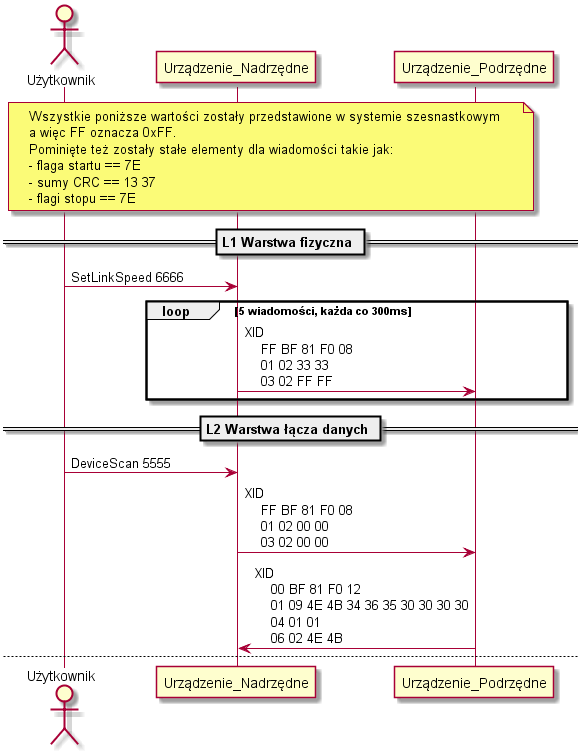
\includegraphics[scale=0.70]{out/Diagramy/UML_DiagramOfSequence_New/UML_DiagramOfSequence_New-page1.png}
        \caption{Ustanowienie prędkości połączenia wraz z początkowym skanowaniem urządzeń
            \newline(Opracowanie własne)}
        \label{fig:DiagramSequence_LinkSpeed_DeviceScan}
        \end{figure}
    \newpage

	Częstą praktyką modelowania etapu łączenia z RET-em jest użycie przy maszyny stanowej w związku z czym, z poniższych funkcjonalności należy korzystać zgodnie z zadaną kolejnością.
	Dla każdej z poniższych ramek wyznaczono część wspólną składającą się z czterech bajtów. Pierwszym z nich jest bajt flagi startu, która oznacza początek wiadomości i ma wartość 0x7E.
	Koleje bajty budują ramkę XID, I, U czy S. Następnie dodaje się dwubajtową sumę CRC oraz na samym końcu flagę stopu, która jest tej samej wartości co flaga startu i oznacza koniec nadawania wiadomości.

    Na diagramach sekwencji przedstawiono komendy wywoływane przez użytkownika
    symulatora wraz z zawartościami ramek pochodzących z urządzenia nadrzędnego oraz
    wartościami ramek przychodzących z urządzenia podrzędnego.
    W celu analizy procesu komunikacji, w opisie skupiono sie na cechach charakterystycznych
    dla poszczególnej ramki czy komendy, o których nie wspomniano we wcześniejszych rozdziałach.
    
    \section{Ustanowienie prędkości połączenia}
    Parametrem tej komendy jest adres portu 6666, z którego korzysta sterownik
    do nawiązania połączenia typu tcp na adresie 127.0.0.1 wraz z symulatorem urządzenia
    przy zastosowaniu wzorca Publish-Subscribe. Podczas tego połączenia protokół AISG 2.0 
    nie zakłada oczekiwania na odpowiedź od urządzenia podrzędnego oraz użyta biblioteka
    ZeroMQ również nie udostępnia możliwości wysłania odpowiedzi na taką wiadomość.
    \newline\newline
	Jest to komenda wysyłana do urządzenia podrzędnego przy pomocy ramki XID.
	\newline
	Pierwsze dwa bajty o wartości 0xFF odpowiadają za zdefiniowanie adresu urządzenia docelowego. 
	W tym przypadku celem jest synchronizacja prędkości połączenia ze wszystkimi urządzeniami na lini, które nie są zaadresowane, a więc jest to wiadomość typu textit{broadcast};
	\newline
	Kolejne dwa bajty kontrolne o wartości 0xBF są charakterystyczne dla ramki XID.
	\newline
	Następne dwa bajty o wartości 0x81 identyfikują format wiadomości XID, co oznacza, że jest to wiadomość z kategorii przypisania adresu.
	\newline
	Potem napotkano kolejne dwa bajty o wartości 0xF0, które są identyfikatorem grupy, co definiuje nam jakie kolejne bajty dopuszczalne są w dalszej części wiadomości.
	\newline
	Urządzenie podrzędne w celu umożliwienia mu zdekodowania wiadomości, otrzymuje w wiadomości długość grupy, czyli dwa bajty w tym przypadku o wartości 0x08 i jest to 
	liczba bajtów która pojawi się następnie, aż do pierwszego bajta sumy CRC.
	\newline
	Przechodząc do przesyłanych parameterów, jako pierwszy będzie to unikalny identyfikator urządzenia. Rozpoznano go po identyfikatorze parameteru o wartości 0x01.
	Następnie podajemy liczbę bajtów zajmowanych przez UniqueID czyli 0x02. Kolejnie podajemy wartość unikalnego identyfikatora. Z racji tego, że nie oczekujemy odpowiedzi
	na tę wiadomość, są to dowolne wartości.
	Drugim przesyłanym parametrem jest maska danych z identyfikatorem o wartości 0x03, potem podajemy liczbę bajtów budujących przesyłaną przez nas maskę czyli 0x02, a w wartości 
	parametru umieszczamy 4-ry bajty o wartości obu 0xFF. Jest to najbardziej ogólna maska urządzenia.

    \section{Skanowanie urządzeń}
    Parametrem tej komendy jest adres portu 5555, z którego korzysta sterownik
    do nawiązania połączenia typu tcp na adresie 127.0.0.1 wraz z symulatorem urządzenia,
    przy zastosowaniu wzorca Żadanie-Odpowiedź. Jest to wzorzec, który zakłada otrzymanie 
    odpowiedzi na każdą wysłaną wiadomość, zanim kolejna zostanie nadana. Opisany mechanizm komunikacji
    aplikowalny jest również do wszystkich poniższych komend.
    Ciekawym elementem tej wiadomości jest to, że otrzymano kod producenta zarówno
    w osobnym parametrze jak i jako składową unikalnego identyfikatora urządzenia.
    \newline\newline
	Budowa ramki wysyłanej przez tę komendę jest bardzo podobna do powyższej z racji tego, że powyższą można nazwać atrapą skanu a tą skanowaniem celowanym.
	Z racji tego, że różna jest liczba oraz wielkość poszczególnych parametrów HDLC, bajt rozmiaru grupy posiada wartość 0x11.
	\newline
	Pierwszy parametr identyfikuje się przy pomocy wartości 0x01 czyli jest to unikalny identyfikator urządzenia, który ma zostać zaadresowany.
	Kolejny bajt przypomina o rozmiarze parametru i w tym przypadku jest on równy 0x09. W powyższym opisie przedstawiono unikalny identyfikator urządzenia, który w przypadku
	równości z rzeczywistym, pozwala urządzeniu podrzędnemu przyjąć żądanie adresacji.
	\newline
	Następny parametr posiada wartość 0x02 i oznacza on, że w jego wartości urządzenie nadrzędne zdefiniowało adres urządzeniu wewnetrznemu, dzięki któremu
	będzie identyfikowane oraz z racji tego, że długość parametru ma wartość 0x01, to wartość wynosi 0x03. W przypadku obecnej pracy, nie będzie miał on większego znaczenia
	aczkolwiek w momencie kiedy urządzenia typu Ret połączone są ze sobą szerogowo, potrzeba jest możliwość wysłania wiadomości do na przykład drugiego w łańcuchu.
	\newline
	Wartość ostatniego parametru równa 0x04, definiuje typ urządzenia podrzędnego, z którym inicjalizowana jest komunikacja. Długość wynosi 0x01 a wartość to 0x01.
	Oznacza ona, że podejmowana jest próba nawiązania komunikacji z pojedyncznym RET-em.
	Dla porównania istnieją również urządzenia takie jak MultiRET, dzięki któremu można zmieniać wartość nachylania kąta głównej wiązki anteny na wielu osiach czy płaszczyznach.

    \section{Żadanie adresacji}
    Tutaj po raz pierwszy można zaobserwować zmienioną wartość pola adresu dla wiadomości
    przychodzącej. Oznacza to, że urządzenie podrzędne zaakceptowało żadanie adresacji 
    oraz identyfikuje się w trakcie rozmowy z urządzeniem nadrzędnym pod adresem 0x03 co
    jest prawdą dla każdej następnej wiadomości.
 
    identyfikujące się unikalnym identyfikatorem \textit{UniqueID} == \{0x4E, 0x4B, 0x34, 0x36, 0x35, 0x30, 0x30, 0x30, 0x30\}

    \begin{figure}[h!]
        \centering
        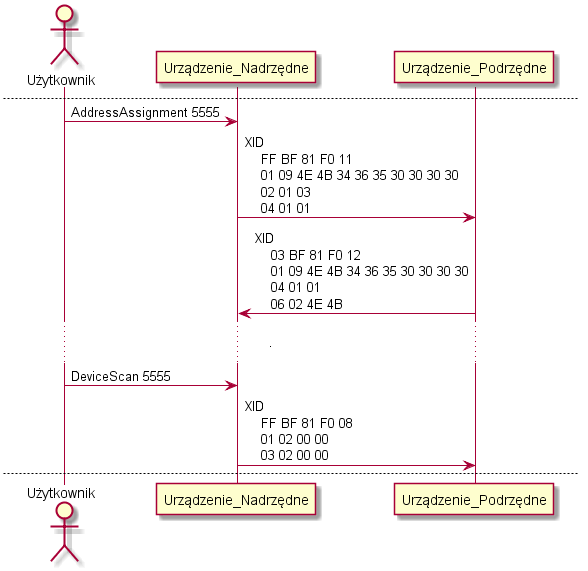
\includegraphics[scale=0.75]{out/Diagramy/UML_DiagramOfSequence_New/UML_DiagramOfSequence_New-page2.png}
        \caption{Żadanie adresacji oraz dodatkowe skanowanie urządzeń.
            \newline(Opracowanie własne)}
        \label{fig:DiagramSequence_AddressAssignment_SecondDeviceScan}
    \end{figure}

    \section{Ponowne skanowanie urządzeń}
    W zakresie tej pracy, komunikacja nawiązywana jest z jednym urządzeniem, a więc dlaczego
    ponownie wysłano wiadomość skanowania ? Otóż na tę wiadomość urządzenie nadrzędne
    nie powinno otrzymać odpowiedzi, gdyż jedynie urządzenia niezaadresowane mogą na nie 
    odpowiedzieć, co jest podstawową metodą dodatkowej weryfikacji powodzenia procedury
    adresowania.

    \section{Negocjacje parametrów HDLC}
    Cechą negocjacji parametrów przy pomocy ramek XID jest to, że jeśli żądana wartość jest wspierana przez
    urządzenie podrzędne, to odpowie ono wiadomością zawierającą te same parametry oraz te same wartości. 
    W przeciwnym wypadku otrzymanymi wartościami parametrów będą największe możliwe przez nie wspierane.
    Zaobserwowano to zjawisko w przypadku negocjacji wielkości payloadu dla wysłanej oraz otrzymanej ramki informacyjnej.
    Urządzenie nadrzędne próbowało ustanowić dopuszczalną liczbę bitów na \{0xF0, 0x2D, 0x00, 0x00\} co daje wartość 61485,
    lecz urządzenie podrzędne odpowiedziało \{0x50, 0x02, 0x00, 0x00\} co po konwersji na system dziesiętny daje 20482 bity.
    \newline\newline
	Teraz można przejść do coraz bardziej szczegółowych parametrów jak ustanowienie numeru wersji standardu 3GPP.
	Podczas tworzenia tej wiadomości znów skorzystano z ramki XID a więc należy zdefiniować identyfikator formatu, grupy oraz jej długość.
    Pierwsze dwie wartości są równe tym z komendy ,,AddressAssignment'' a długość ma wartość 0x03.
	Identyfikatorem parametru jest tym razem wartość 0x05, długością 0x01 natomiast wartościa parametru 0x08.
    Jest to wersja standardu w wersji 8-mej czyli pionierska dla technologii \textit{LTE}.
	Wprowadzono w niej wparcie dla interfejsu radiowego opartego o \textit{OFDMA}, którego wykorzystanie można zaobserwować również przy technologii 5G.
    \newline\newline
	Powyższą wiadomość można rozbić na 4-ry osobne aczkolwiek połączono je z racji podobnych funkcjonalności realizowanych podczas jej wysłania.
    Protokół AISG bazuje na HDLC, które używane jest w wielu miejscach
	gdzie potrzebne jest połączenie połączenie o wysokiej gwarancji otrzymania wiadomości bez utraty informacji.
    Istnieje nawet jego realizacja służąca do komunikacja satelit kosmicznych i różni się ona od AISG głównie
	ustalonymi wiadomościami HDLC, gdzie potrzeba wysłać znacznie większą liczbę ramek na raz aniżeli tylko jedna.
	Pierwszy bajt adresu może zostać zmieniony z wartości 0xFF na 0x03, gdyż w poprzedniej wiadomości ustanowiono adres urządzenia podrzędnego.
    Ta wartość będzie aplikowana do każdej poniższej wiadomości a więc pominięto jej wspominanie,
	gdyż potraktowano ją jako stałą.

    Z racji tego, że implementowana wersja protokołu AISG 2.0 jest jedną z wielu ( istnieją jeszcze dwie wcześniejsze: 1.0, 1.1 oraz najnowsza 3.0),
    potrzeba zdefiniować według którego standardu budowane są przez urządzenie nadrzędne oraz rozpoznawane przez podrzędne.
	Bajt identyfikujący parametr dla tej wiadomości ma wartość 0x14, długość parametru to 0x01 a jej wartość to 0x02.
	\newline
	Następnym bajtem jest identyfikator formatu, który dla wiadomości zawierającej parametry HDLC jest równy 0x81.
	\newline
	Kolejny bajt czyli identyfikator grupy ma wartość 0x80, a następny (rozmiar grupy) jest równy 0x12.
	\newline
	Pierwszym parametrem HDLC który jest negocjowany to maksymalny rozmiar \textit{payloadu} dla ramki informacyjnej nadawanej przez urządzenie nadrzędne.
    Identyfikatorem w tym przypadku jest 0x05. Rozmiar payloadu jest równy 0x04 a wartościami są \{ 0xF0, 0x2D, 0x00, 0x00 \}.
	\newline
	Kolejny bajty natomiast budują negocjowany maksymalny rozmiar payloadu ramki informacyjnej do wiadomości otrzymywanej przez urządzenie nadrzędne.
    Identyfikator ma wartość 0x06 a pozostały bajty są tożsame jak dla poprzedniej
	negocjacji.
	\newline
	Następnym parametrem jest maksymalna liczba ramek wysłanych pod rząd przez urządzenie nadrzędne. Identyfikator ma wartość 0x07 a zarówno długość jak i wartość to 0x01.
	\newline
	Ostatnim parametrem negocjowanym podczas tej wiadomości jest maksymalna liczba ramek otrzymanych pod rząd poprzez urządzenie nadrzędne.
    Wartość identyfikatora jest równa 0x08 a długość oraz wartość znów posiadają wartości 0x01.

    \section{Przejście na normalny tryb komunikacji}
    Jako odpowiedź na tę wiadomość urządzenie otrzyma ramkę, która zawiera wartość 0x73, co oznacza że 
    potwierdza ono żądane oczekiwanie.
    \newline\newline
	Bajt kontrolny posiada wartość 0x93 i oznacza żadanie ustalenia sposobu komunikacji z urządzeniem podrzędnym na tryb normalny, 
    a więc taki w którym wysyła ono ramkę jedynie jako odpowiedź na wcześniej nadaną przez urządzenie nadrzędne.

    \section{Kalibracja}
    Po pomyślnym zestawieniu warstwy fizycznej posiadamy zdefiniowany wszystkie charakterystyki połączenia, 
    które pozwolą w jednoznaczny sposób porozumieć sie z urządzeniem oraz żądać odpowiedzi na wysłaną wiadomość.
	Kolejne komendy są już żądaniami wysokoziomowymi, które definiują użyteczne dla klienta polecenia służąca do zarządzania RET-em.
    Jest ich znacznie więcej, aczkolwiek obranym celem pracy inżynierskiej było pomyślne przeprowadzenie kalibracji urządzenia, 
    co pozwala w dalszym etapie ustawić zadany kąt odchylenia głównej wiązki sygnału z anteny.

    W związku z tym, że oczekiwanie kalibracji przesłano przy pomocy ramki informacyjnej, bajt kontrolny posiada
    charakterystyczną metodę jego ewaluacji przedstawioną wcześniej. Diagram sekwencji
    potwierdza to, gdyż wiadomość odebrana przez urządzenie nadrzędne posiada wartość równą 0x30.
    Ramka odebrana, na wyznaczenie liczby bajtów budujących odpowiedź posiada zarezerowane dwa bajty. 
    Ciekawą obserwacją jest to, że odpowiedź równą 0x00 czyli OK można by zapisać przy pomocy jedynie jednego bajta, lecz optymalizacja
    pamięci nie jest tutaj zastosowana.
    \newline\newline
	Z racji tego, że wiadomości tej warstwy korzystają z ramki informacyjnej, inną rolę pełni bajt kontrolny. Poza stałymi wartości bitów w bajcie 
	każdorazowe wysłanie i odebranie wiadomości zmienia wartość sekcji P/F wcześniej wspomnianej. 
	Dzięki temu można w łatwy sposób identyfikować czy wiadomość, którą otrzymujemy jest ta której oczekiwaliśmy. 
	W związku z tym dla pierwszej wiadomości wysłanej przez urządzenie nadrzędne poprawną wartością będzie 0x10.
	\newline
	Kolejnym bajtem jest kod procedury, który ma wartość 0x31, co oznacza, że oczekujemy kalibracji urządzenia będącego zwykłym pojedynczym RET-em.
	\newline
	Z racji tego, że podczas tej komendy nie jest przesyłana żadna wartość dla tej procedury, dwa bajty zaalokowane dla długości parametru mają wartość \{0x00, 0x00\}

    \begin{figure}[h!]
        \centering
        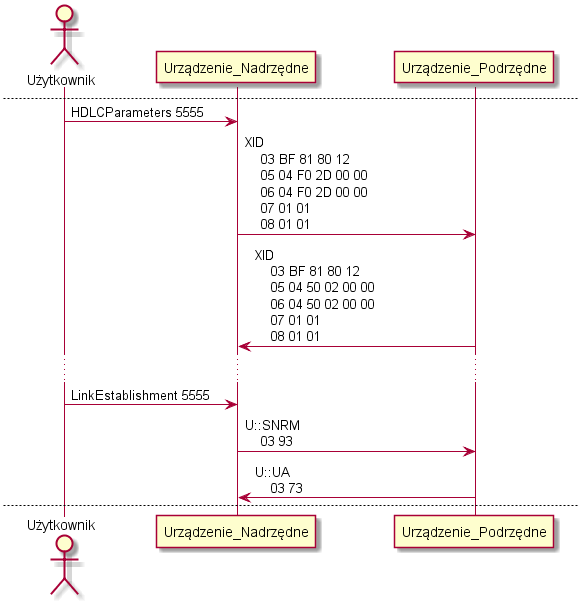
\includegraphics[scale=0.75]{out/Diagramy/UML_DiagramOfSequence_New/UML_DiagramOfSequence_New-page3.png}
        \caption{Negocjacja rozmiaru okna oraz payloadu ramki informacyjnej oraz ustanowienie normalnego trybu komunikacji.
            \newline(Opracowanie własne)}
        \label{fig:DiagramSequence_HDLCParameters_SNRM}
    \end{figure}

    \begin{figure}[h!]
        \centering
        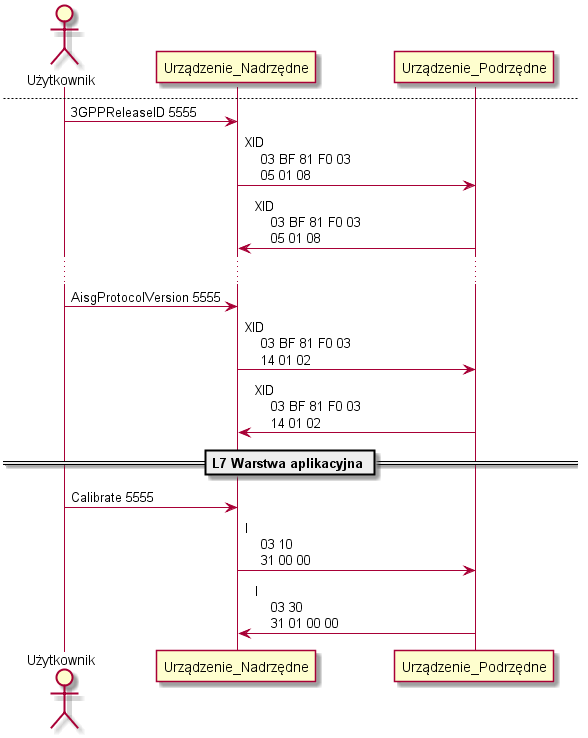
\includegraphics[scale=0.75]{out/Diagramy/UML_DiagramOfSequence_New/UML_DiagramOfSequence_New-page4.png}
        \caption{Negocjacja pozostałych parametrów HDLC oraz żadanie kalibracji urządzenia.
        \newline(Opracowanie własne)}
        \label{fig:DiagramSequence_3GPP_AISGVersion_Calibrate}
    \end{figure}
